\documentclass[12pt, a4paper]{article}

% Geometry and Layout
\usepackage[a4paper, margin=1in]{geometry}
\usepackage{indentfirst} % Indent first sentence of a new section.
\usepackage{ntheorem}
\theoremseparator{:}
\newtheorem{hyp}{Hypothesis}
% Line Spacing
\usepackage{setspace}
\doublespacing

% Fonts

% Bibliography and Citations
\usepackage[authoryear,round]{natbib} % authoryear and round are for APA-style citations
\bibliographystyle{apalike} % APA-like style for the bibliography

% Math & Equations
\usepackage{amsmath}

% Tables & Figures
\usepackage{tabularx, booktabs, graphicx}

% Other Packages
\usepackage{hyperref, float, caption}

\begin{document}

\title{Digital Research Seminar: \\ Green Metrics: How are Sustainable Bonds characterized?}
\author{
    Patrick Röthlisberger\thanks{ZHAW (Institute for Financial Management), email: patrick.roethlisberger@zhaw.ch}
    \and
    Stefan Aebi\thanks{xxx, email: aebystefan@gmail.com}
    }
\date{\today} % or specify a date like \date{September 29, 2023}
\maketitle

\begin{abstract}
In this document we document our project to describe sustainable bonds and their emitting companies. This is meant to be done on a yearly basis and can be used to introduce papers on that topic or it can be shown in lectures.
\end{abstract}
\newpage
\tableofcontents
\newpage
\section{Introduction}
Sustainable debt security instruments (bonds) are increasingly becoming one focus of the extensive sustainable finance discussion worldwide. Bonds with a specific, sustainable purpose (e.g. Green Bonds (GB)) as well as bonds with a general purpose but linked to one or more sustainability goals (Sustainability Linked Bonds (SLBs)) are becoming increasingly popular on the capital market (as shown in figure 1). The decline in 2022 is due to the overall difficulties in the bond market due to increasing interest rates \citep{Sgrue2023sustainable-bond-issuance}. An important driver of this trend over the last two years is the demand from the (private-) investor side \citep{pietschPricingGreenBonds2022}.

\section{Goal}
In this project, we try to find differences in the sustainable bonds and the financials of the issuing companies. The main question is if there is a conection between the type of sustainable bond and the financial performance, size, cash flow, and profitability. The biggest challange for this project is that data availability is restricted to users with access to common data providers, like Bloomberg or Refintitv Eikon. First, we therefore document the process of fetching the data from these platform for others to update or recreate our findings. Secondly, we provide the data downloaded on the date of this project for those without access to the data platforms.

\section{Data}
Data initially comes from the Bloomberg terminal. We created the following search conditions:
\begin{itemize}
    \item Bonds: All
    \item (and) BICS Classification: Exclude Sovereigns, or Government, Regional Government, Supranational, State Development Banks, Liquidation Agencies, or Central Banks, or Local Government.
    \item (and) Green Instrument - Indicator as Yes
    \item (or) Social Instrument - Indicator as Yes
    \item (or) Sustainability Linked Indicator as Yes
    \item (and) Emission Date later than 12/31/2014
    \item (and) Country/Region of Issuance including Europe
\end{itemize}
The resulting data is then downloaded to \textit{Excel (OR DO WE MAKE A CSV FILE??)} and expanded with an additional column including an identifier for the issuer and other columns for further bond indicators. The file can be found in the downloads. The identifier is then used to create additional columns with the financials of the issuer. As several issuers are unlisted financial subsidiaries we need the data for the parent company. We use the Refinitiv Eikon database to get the ultimate parent identifier and the required financial one year before the bond issuance. The following table shows the structure and the code used in Excel. Fetching data from Refintitv Eikon for a specific date in each row is not possible with the Refintitv API in Python (see Appandix to see an Example API and data fetching). The basic formula looks like this: 
\begin{align}
    =RDP.Data(Identifier Cell Reference;"Code";"Sdate=\#1";;Date Cell Reference)
\end{align}

The data frame includes numbers for size, profitability, leverage, and cash flow (italic are the Refinitiv codes):

\begin{itemize}
    \item \textbf{Emission Date -1}
    \item \textbf{Total Assets}: \textit{TR.F.TotAssets} in Emission Date -1
    \item \textbf{Market Cap:} \textit{TR.CompanyMarketCapitalization} in Emission Date -1
    \item \textbf{Tobins Q: }Tot.Assets divided by CompanyMarketCapitalization
    \item \textbf{Leverage:} \textit{TR.PCLTDebtToTotEquPct} in Emission Date -1
    \item \textbf{Cash Flow to total Assets:} \textit{TR.F.NetCFOpToTotAssets} in Emission Date -1
    \item \textbf{Return on Asset (ROA):} \textit{TR.F.ReturnAvgTotAssetsPctTTM} in Emission Date -1
    \item \textbf{Return on Equity (ROE):} \textit{TR.F.ReturnAvgComEqPctTTM} in Emission Date -1
    \item \textbf{TRBC Economic Sector:} \textit{TR.TRBCEconomicSector} of Parent
    
\end{itemize}

The numbers catched with the codes is then copied and saved in a final static file so there are no more codes involved (this is due to performance issues when working with Refinitiv codes in Excel).

\section{Results}
\subsection{Market Overview}
As seen in Figure \ref{fig:market}, we can see a growing market of sustainable bonds overall in Europe. The decline in 2022 is not due to lower interest in the products but rather due to the difficult interest and market situation. Still, in 2022 the market share of sustainable bonds in Europe is still lower than 10\%. 
\begin{figure}[H]
    \centering
    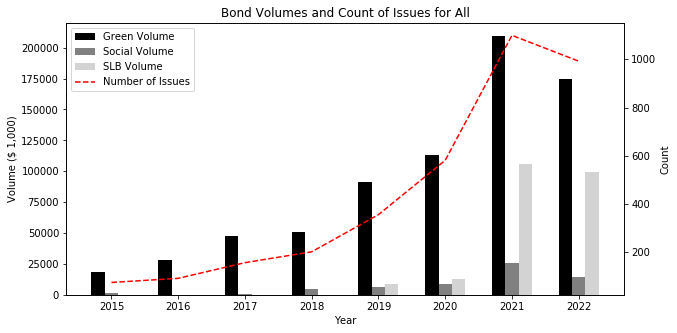
\includegraphics[width=1\linewidth]{VolumeCount.png}
    \caption{Sustainable Bonds Emissions in Europe (Data from Bloomberg)}
\label{fig:market}
\end{figure}

\subsection{Bond Metrics}

Table \ref{table:1} gives a short overview on the numbers on Coupon (Kpn), Emission Volume (Ausg\_Mge) and Maturity while table \ref{table:2} is giving the number of outstanding bonds for each category:

\begin{table}[htbp]
\centering
\begin{tabular}{lll}
    \toprule
    {} & mean & std \\
    \midrule
    Ausg\_Mge & 300,412,618.30 & 348,381,822.82 \\
    Kpn & 2.67 & 2.49 \\
    Maturity & 7.43 & 16.68 \\
    \bottomrule
\end{tabular}
\caption{Table with summary statistics}
\label{table:1}
\end{table}

\begin{table}[htbp]
\centering
\begin{tabular}{ll}
\toprule
Green Instrument & 3301 \\
Social Bond & 199 \\
Sust Linked & 580 \\
\bottomrule
\end{tabular}
\caption{Table with number of outstanding bonds}
\label{table:2}
\end{table}

The following graphs show more graphical insights on how the three indicators are different in each instrument and over time. Each of the analysis can be adjusted and filtered for a certain country or industry.

\begin{figure}[H]
    \centering
    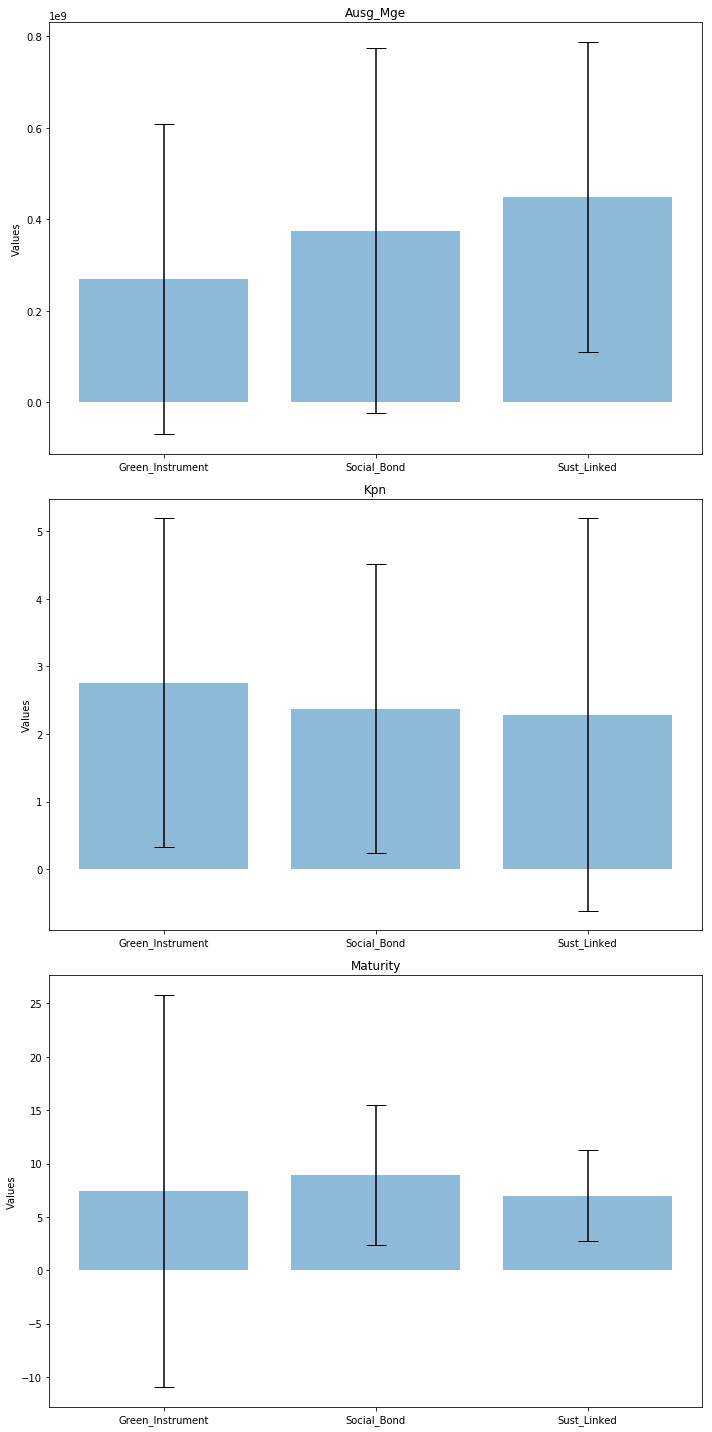
\includegraphics[width=0.8\linewidth, height=0.8\textheight, keepaspectratio]{Metrics_per_Bond.png}
    \caption{Coupon, Emission Volume and Maturity for each Bond Category}
\label{fig:Metrics}
\end{figure}

\begin{figure}[H]
    \centering
    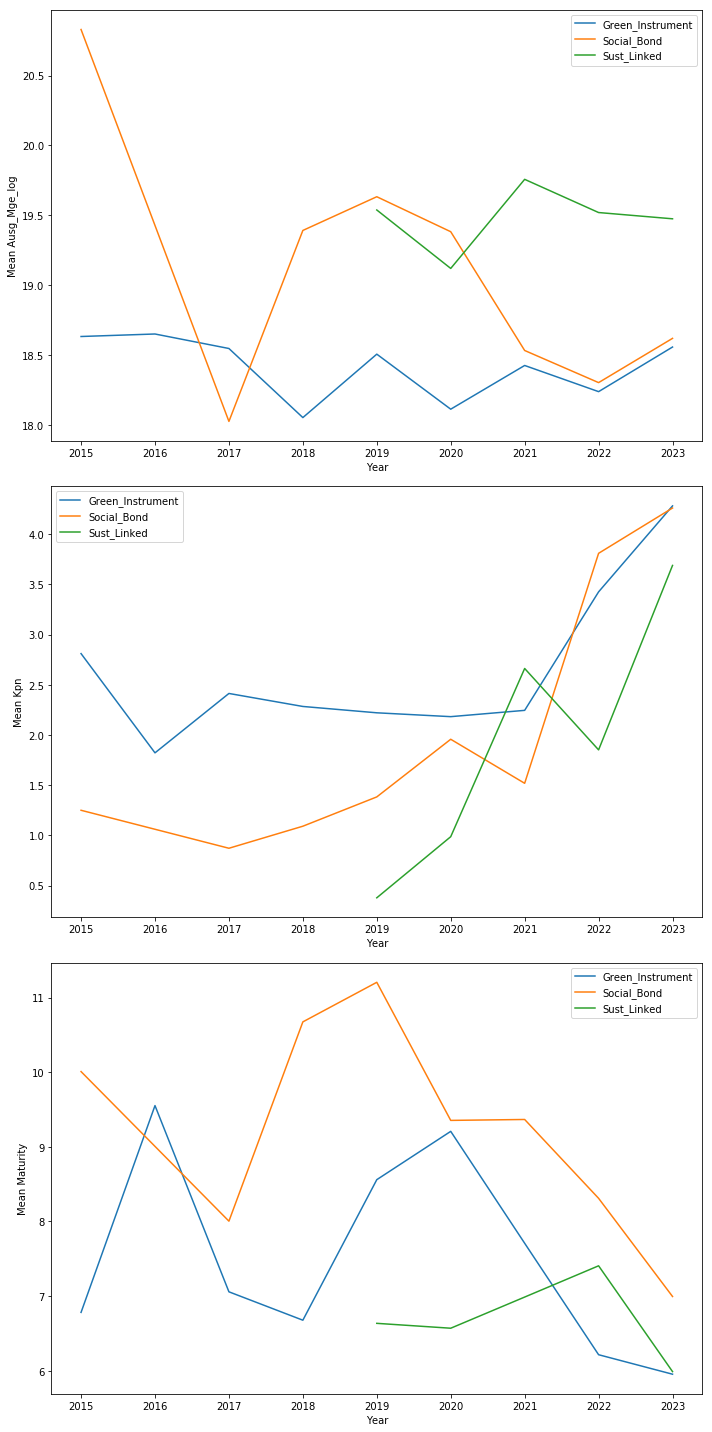
\includegraphics[width=0.8\linewidth, height=0.8\textheight, keepaspectratio]{Metrics_overtime.png}
    \caption{Coupon, Emission Volume and Maturity over time}
\label{fig:MetricsTime}
\end{figure}

\subsection{Company Financials}
In this section we analyzed what the differences in the companies who issue sustainable bonds are. First we can see in table \ref{table:3} which industries issue sustainable bonds. Financials are on top, which is normal (when we do not measure the parent companies, those values would be even higher as many companies use their financial subsidiary for a bond issue). Tables \ref{table:4} to \ref{table:6} show the financial differences in the different instruments.

\begin{table}[h]
\centering
\caption{Industry Counts}
\begin{tabular}{lr}
\hline
Industry & Count \\
\hline
Financials & 351 \\
Utilities & 176 \\
Industrials & 109 \\
Real Estate & 101 \\
Basic Materials & 44 \\
Consumer Cyclicals & 44 \\
Technology & 25 \\
Consumer Non-Cyclicals & 23 \\
Energy & 16 \\
Healthcare & 10 \\
\hline
\end{tabular}
\label{table:3}
\end{table}

\begin{table}[h]
\centering
\caption{Green Instrument Statistics}
\begin{tabular}{lrrrrr}
\hline
 & TobinsQ & LTLeverage & CFtoAsset & ROA & ROE \\
\hline
count & 723.00 & 723.00 & 723.00 & 723.00 & 723.00 \\
mean & 0.39 & 147.48 & 0.03 & 2.46 & 9.53 \\
std & 0.99 & 129.69 & 0.04 & 3.43 & 9.93 \\
min & 0.00 & 0.00 & -0.07 & -9.20 & -34.39 \\
25\% & 0.05 & 71.50 & 0.01 & 0.45 & 5.49 \\
50\% & 0.22 & 117.21 & 0.03 & 1.32 & 8.86 \\
75\% & 0.41 & 158.68 & 0.06 & 3.11 & 12.02 \\
max & 16.82 & 1016.25 & 0.21 & 20.22 & 65.38 \\
\hline
\end{tabular}
\label{table:4}
\end{table}

\begin{table}[h]
\centering
\caption{Social Bond Statistics}
\begin{tabular}{lrrrrr}
\hline
 & TobinsQ & LTLeverage & CFtoAsset & ROA & ROE \\
\hline
count & 37.00 & 37.00 & 37.00 & 37.00 & 37.00 \\
mean & 0.21 & 128.00 & 0.03 & 2.35 & 11.24 \\
std & 0.25 & 68.26 & 0.04 & 2.71 & 7.29 \\
min & 0.01 & 14.90 & -0.02 & 0.03 & -1.23 \\
25\% & 0.03 & 91.99 & -0.00 & 0.39 & 6.36 \\
50\% & 0.06 & 120.99 & 0.02 & 0.70 & 9.02 \\
75\% & 0.34 & 138.39 & 0.05 & 5.62 & 15.21 \\
max & 0.95 & 382.56 & 0.14 & 9.75 & 32.97 \\
\hline
\end{tabular}
\label{table:5}
\end{table}

\begin{table}[h]
\centering
\caption{Sustainability Linked Statistics}
\begin{tabular}{lrrrrr}
\hline
 & TobinsQ & LTLeverage & CFtoAsset & ROA & ROE \\
\hline
count & 139.00 & 139.00 & 139.00 & 139.00 & 139.00 \\
mean & 3.31 & 100.37 & 0.07 & 2.53 & 7.27 \\
std & 20.24 & 56.29 & 0.04 & 4.82 & 15.60 \\
min & 0.03 & 0.10 & 0.00 & -12.19 & -48.28 \\
25\% & 0.33 & 61.69 & 0.05 & 1.75 & 5.76 \\
50\% & 0.48 & 112.65 & 0.07 & 2.16 & 8.60 \\
75\% & 0.63 & 117.00 & 0.08 & 4.14 & 11.97 \\
max & 169.55 & 375.29 & 0.32 & 21.60 & 81.53 \\
\hline
\end{tabular}
\label{table:6}
\end{table}

\clearpage

\begin{figure}[H]
    \centering
    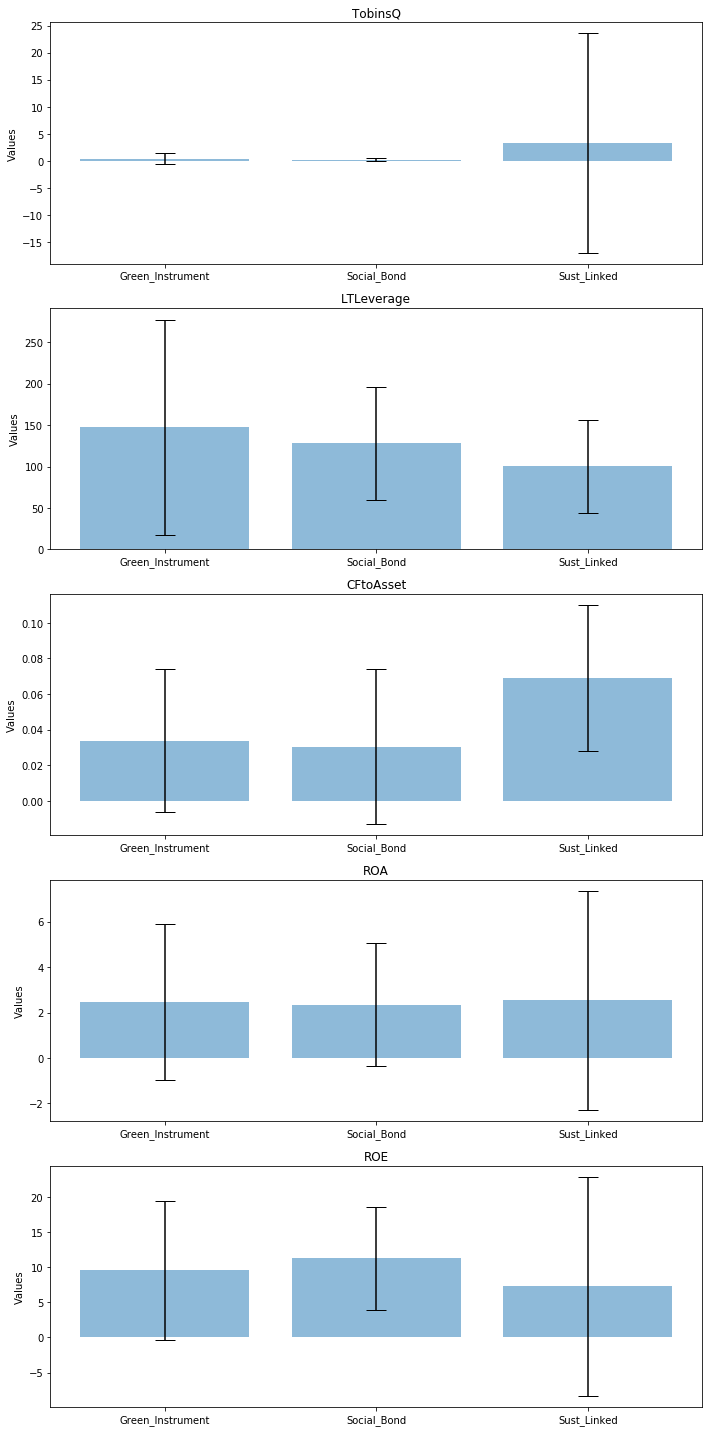
\includegraphics[width=0.8\linewidth, height=0.8\textheight, keepaspectratio]{Company_Data.png}
    \caption{Company Data}
\label{fig:CompanyData}
\end{figure}

\begin{figure}[H]
    \centering
    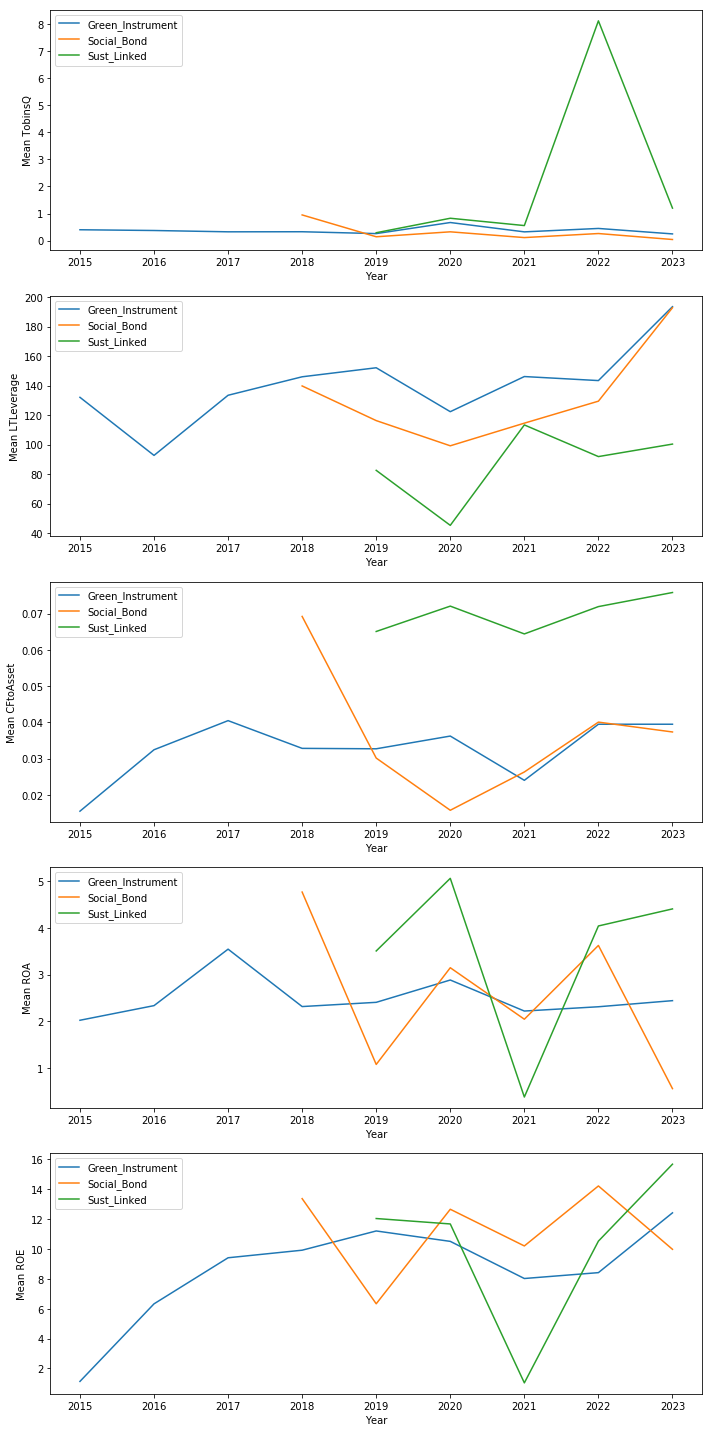
\includegraphics[width=0.8\linewidth, height=0.8\textheight, keepaspectratio]{Company_Data_overtime.png}
    \caption{Company Data over time}
\label{fig:CompanyTime}
\end{figure}

\newpage

% The bibliography
\bibliography{Meine_Bibliothek}

\section{Appendix}
\subsection{Refinitiv Workspace Python API}
\begin{itemize}
    \item Open Refintitv Workspace
    \item Select the API Key Generator in the APPLIP
    \item 2. Select the Eikon Data API's tick box as the API Type
    \item Click the ‘Register’ New App button
\end{itemize}
\end{document}
